\problemname{Ett markant problem}


\begin{center}
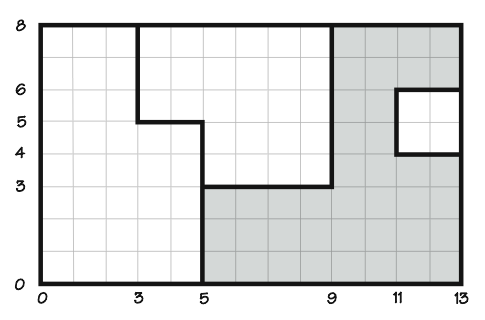
\includegraphics[width=0.6\textwidth]{markant.png}
\end{center}

Storbonden Sven äger ett stort staketinhägnat rektangulärt område mark. Han har låtit dela upp marken i flera mindre områden genom att bygga staket så att varje mindre område är helt inhägnat av staket. Samtliga staket är raka och placerade parallellt med ytterkanterna. Nu ska Svens äldste son, Peter, gifta sig, och som bröllopspresent kommer han då få ett av dessa mindre områden. Peter vill självfallet ha det största området (sett till arean), men då Sven har varit klurig och delat in sin mark på ett komplicerat sätt är det inte helt enkelt att avgöra vilket område som är störst. Hjälp Peter att lösa problemet genom att skriva ett program som beräknar vilken del som har störst area.



\section*{Indata}
Den första raden innehåller tre heltal, $b, h$ ($0 < b, h \le 40000$) och $n$ ($4 \le n \le 50$),
där $b$ och $h$ anger bredden respektive höjden på Svens markområde och $n$ anger antalet staket på Svens mark.

Därefter följer $n$ stycken rader med fyra heltal på varje rad, $x_1$, $y_1$, $x_2$, $y_2$
($0 \le x_1$, $x_2 \le b$ och $0 \le y_1, y_2 \le h$) som anger start- och ändpunkten på ett staket.
Det nedre vänstra hörnet på Svens område har koordinaterna $(0, 0)$ och det övre högra koordinaterna $(b, h)$.
Du kan anta att de fyra staketen, som inhägnar hela Svens område, är med i listan över staket,
samt att inga staket korsar eller överlappar varandra.

\section*{Utdata}
Skriv ut ett heltal: arean av det största området.


\section*{Poängsättning}
Din lösning kommer att testas på flera testfall. För att få 100 poäng så måste du klara alla testfall.



